% ============================================================================
%  Filter-Aware Face Manipulation Detection on Edge Devices
%  Rewritten 2026-09-06 from the 2026-08 draft.
%
%  EVERY number in this file is traceable to a file under results/ that can be
%  recomputed.  Numbers that are not yet measured appear as \TODO{...} and MUST
%  NOT be replaced by estimates.  See docs/DRAFT_AUDIT_20260906.md for the audit
%  of the previous draft (three claims were withdrawn, one table had no source).
% ============================================================================
\documentclass[conference]{IEEEtran}
\IEEEoverridecommandlockouts

\usepackage{cite}
\usepackage{amsmath,amssymb,amsfonts}
\usepackage{graphicx}
\usepackage{booktabs}
\usepackage{multirow}
\usepackage{xcolor}
\usepackage{url}
\usepackage[hidelinks]{hyperref}
\usepackage{tikz}
\usetikzlibrary{arrows.meta,positioning,fit,calc}
\graphicspath{{figs/}}

% Pending results -- must be visibly ugly so they cannot be forgotten.
\newcommand{\TODO}[1]{\textcolor{red}{\textbf{[TODO: #1]}}}
\newcommand{\ours}{\textsc{Ours}}
\def\BibTeX{{\rm B\kern-.05em{\sc i\kern-.025em b}\kern-.08em T\kern-.1667em\lower.7ex\hbox{E}\kern-.125emX}}

\begin{document}

\title{Beauty Filters Are a Third Class:\\
Filter-Aware Face Manipulation Detection on Edge Devices}

\author{\IEEEauthorblockN{Qin-Ying Lin, Bo-Rong Chen, Chen-Shan Yu}
\IEEEauthorblockA{\textit{Advisor: Prof. Shang-Hong Lai}\\
\textit{National Tsing Hua University}}}

\maketitle

\begin{abstract}
Face manipulation detectors are almost universally trained and evaluated as binary
real-versus-fake classifiers. Yet one in five adults routinely applies beauty filters to
their own photographs, and such retouching is neither authentic capture nor malicious
forgery. We show that this omission is not a detail but a structural defect. Under a
single protocol on identical images, we find that applying four ordinary beauty filters to
genuine faces drives the false-accusation rate of \emph{every} one of eleven published
detectors from below five percent to between 22.5\% and 33.7\%, at a matched operating
point; the same failure mode is absent from a detector that treats filtering as its own
class, which reaches 0.0\%. Crucially, our own architecture trained in the conventional
binary manner reproduces the 23.3\% failure, isolating the label space rather than the
backbone as the cause. In a controlled experiment in which four detectors share backbone, data, recipe and
seed and differ \emph{only} in their label space, no threshold on any binary variant ---
nor on any of the eleven published detectors --- attains both a lower false-accusation
rate and a lower miss rate on filtered fakes than the three-way model.
We further contribute the first
same-protocol comparison of published detectors under filter-aware evaluation
(thirteen models, 13{,}026 images, three protocols, all with cluster-bootstrap
confidence intervals), a hierarchical three-way detector that runs in
\SI{43}{\milli\second} per image on a desktop CPU at 5.06\,M parameters, and an honest
account of where the approach fails: on a third-party beautification benchmark our
detector is outperformed by several of the baselines, and we trace that failure to a
specific, countable corpus shortcut in our own training data.
\end{abstract}

\begin{IEEEkeywords}
face forgery detection, beauty filters, retouching detection, explainability,
edge deployment, benchmark
\end{IEEEkeywords}

% ============================================================================
\section{Introduction}
% ============================================================================

Generative models now synthesise facial imagery that humans identify correctly only about
a quarter of the time~\cite{groh2022}. The forensic response has converged on a binary
formulation: given a face, decide \emph{real} or \emph{fake}. This formulation contains an
assumption that is false in practice --- that every image is either an untouched capture or
a malicious forgery.

A very large fraction of the face images actually circulating online occupy a third
category. Beauty filters --- skin smoothing, whitening, eye enlargement, face slimming ---
are applied by ordinary users to their own photographs. They alter texture and geometry
while \emph{preserving identity}, and they are neither authentic nor forged in the sense a
forensic system cares about. A binary detector must nevertheless assign them to one of its
two labels, and either choice is wrong: calling them \emph{real} concedes that manipulated
pixels are undetectable, and calling them \emph{fake} accuses an ordinary user of forgery.

Saeed \emph{et al.}~\cite{saeed2025} recently showed that beauty filters can be used
adversarially, letting manipulated faces evade detection. We show that the converse
failure is at least as damaging and has not previously been measured: filters cause
detectors to \emph{falsely accuse genuine faces}. On identical images at a matched
operating point, all eleven published detectors we evaluate move from below 5\% to
22.5--33.7\% false accusation once a filter is applied (Section~\ref{sec:p3}).

\begin{figure*}[t]
\centering
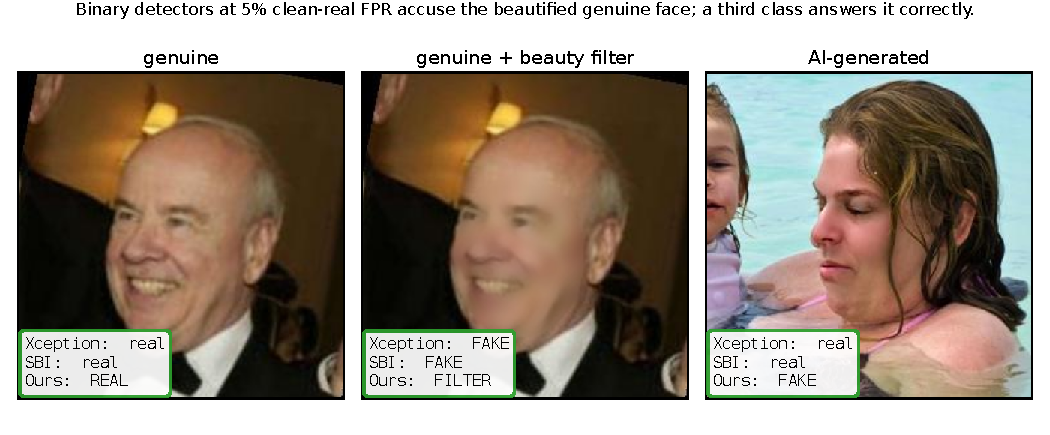
\includegraphics[width=\textwidth]{fig_teaser.pdf}
\caption{\textbf{The failure mode this paper measures.} A genuine face (left), the same face
after an ordinary skin-smoothing filter (centre), and an AI-generated face (right), with the
verdict of two published binary detectors and of our three-way detector, all read at a
matched 5\,\% false-positive rate on clean genuine faces. The binary detectors accept the
genuine face and then accuse it once it is beautified; the three-way detector assigns it to
\emph{filter} --- an answer the binary label space cannot express. Images are from the
held-out True Test split and the verdicts are taken verbatim from the per-image score files
released with the benchmark.}
\label{fig:teaser}
\end{figure*}

We argue --- and test --- that this is a property of the label space, not of any particular
model. Our contributions are:

\begin{enumerate}
\item \textbf{A measured, bidirectional characterisation of the filter problem.} We
      quantify both failure directions on the same images, under one protocol, with
      confidence intervals: filters hiding fakes, and filters causing false accusation of
      real faces (Sections~\ref{sec:p1}--\ref{sec:p3}).
\item \textbf{The first same-protocol, filter-aware benchmark of published detectors.}
      Thirteen models (eleven published, two of our own training regimes) scored on
      13{,}026 identical images across three protocols, with each model's official
      pre-processing and both its published and a threshold-matched operating point.
      Per-image scores are released.
\item \textbf{Evidence that the third class is necessary, not merely convenient.}
      Our own architecture trained conventionally fails exactly like the published
      detectors (23.3\%), while the three-way version reaches 0.0\%. A four-arm controlled
      experiment isolating the label space confirms that no binary operating point matches
      the three-way model on both axes (Section~\ref{sec:necessity}).
\item \textbf{A deployable detector, with its costs stated.} 5.06\,M parameters,
      \SI{20.6}{\mega\byte}, \SI{43}{\milli\second} per image on a desktop CPU ---
      a median of $4.3\times$ fewer parameters and $7.1\times$ faster than the published
      detectors --- including a reformulation of the frequency branch that makes it
      exportable to mobile runtimes at all (Section~\ref{sec:deploy}).
\item \textbf{A negative result we did not have to report.} On the third-party Celeb-DF-B
      beautification benchmark our detector loses to several baselines, and we identify
      the cause as a countable corpus shortcut in our own training data
      (Section~\ref{sec:celebdfb}).
\end{enumerate}

% ============================================================================
\section{Related Work}
% ============================================================================

\subsection{Binary face forgery detection}
The dominant line of work treats detection as binary classification over a forgery corpus.
Xception on FaceForensics++~\cite{rossler2019} remains the reference baseline; subsequent
work adds frequency cues (F3Net~\cite{qian2020}, SPSL~\cite{liu2021}, SRM~\cite{luo2021}),
reconstruction objectives (RECCE~\cite{cao2022}), disentanglement (UCF~\cite{yan2023ucf}),
or consistency regularisation (CORE~\cite{ni2022}). A second family avoids forgery corpora
altogether: SBI~\cite{shiohara2022} trains only on self-blended versions of real images,
and UnivFD~\cite{ojha2023} and NPR~\cite{tan2024} target generator-agnostic cues. None of
these define a class for identity-preserving retouching. We evaluate all of them.

\subsection{Retouching and filter detection}
RetouchingFFHQ~\cite{ying2023} is the first large-scale retouching benchmark and defines the
four cosmetic operations we adopt. It formulates the task as multi-label, multi-level
prediction rather than as a class within a forgery detector, and does not measure the
interaction with forgery detection. Saeed \emph{et al.}~\cite{saeed2025} measure filters as
an evasion attack on deepfake detectors. Our formulation differs in placing filtering
inside the detector's own label space and in measuring both failure directions.

\subsection{Explainability for forensics}
FakeShield~\cite{xu2025} and FakeVLM~\cite{wen2025} produce natural-language artifact
explanations using multimodal LLMs, at a cost (7.24\,GB of VRAM and roughly ten seconds per
image in our own measurement of FakeVLM) that precludes on-device use. Gradient attribution
methods such as Grad-CAM++~\cite{chattopadhyay2018} are cheap but must be sanity-checked:
Adebayo \emph{et al.}~\cite{adebayo2018} show that saliency maps can be insensitive to model
parameters. We apply that check to our own system and report a null result
(Section~\ref{sec:xai}).

\subsection{Efficient backbones}
ShuffleNetV2~\cite{ma2018}, MobileNet-family and EfficientNet-Lite architectures target
mobile inference. We benchmark four candidates before selecting one (Table~\ref{tab:backbone}),
and later re-examine that choice under a different protocol (Section~\ref{sec:limits}).

% ============================================================================
\section{Method}
% ============================================================================

\begin{figure*}[t]
\centering
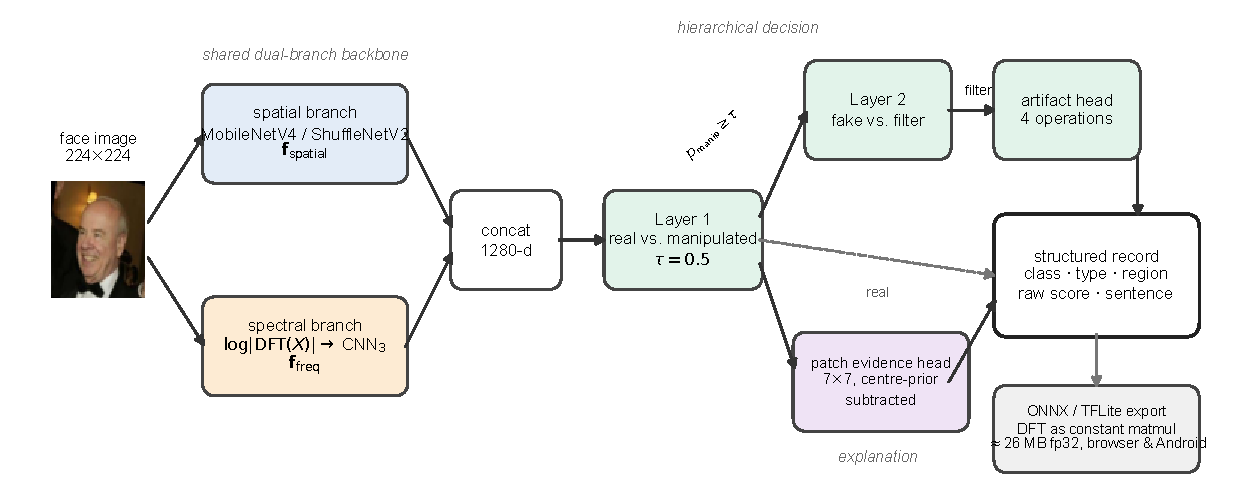
\includegraphics[width=\textwidth]{fig_pipeline.pdf}
\caption{\textbf{System overview.} A dual-branch backbone (spatial + spectral) feeds an
explicit-threshold hierarchical decision: real versus manipulated first, then fake versus
filter, with an artifact-type head for filters. A trained patch evidence head produces the
region claim after subtracting the centre-prior baseline; the output is a structured record,
not free text. The spectral DFT is exported as a constant matrix product so the whole graph
uses standard operators on mobile runtimes (Sec.~\ref{sec:deploy}).}
\label{fig:arch}
\end{figure*}

\subsection{Semantic class definition}
Our taxonomy is defined by \emph{semantics}, not by generation algorithm:

\begin{itemize}
\item \textbf{real}: unmodified capture.
\item \textbf{fake}: identity replacement or full synthesis (face swapping, GAN, diffusion).
      Reenactment belongs here: the content is fabricated.
\item \textbf{filter}: identity-preserving beautification --- smoothing, whitening, eye
      enlargement, face reshaping.
\end{itemize}

The distinction is deliberately independent of implementation. A commercial beautification
app that internally uses a neural network still produces a \emph{filter} output, because
identity is preserved.

\subsection{Dual-branch backbone}
Mild cosmetic filters attenuate high-frequency texture and shift colour statistics without
altering geometry, which spatial CNNs handle poorly. We therefore combine a spatial and a
spectral stream. For an input $X$,
\begin{align}
\mathbf{f}_{\mathrm{spatial}} &= \mathrm{ShuffleNetV2}(X) \in \mathbb{R}^{1024},\\
\mathbf{f}_{\mathrm{freq}} &= \mathrm{CNN}_3\!\left(\log\left|\mathcal{F}(X)\right|\right)
   \in \mathbb{R}^{256},
\end{align}
concatenated to $\mathbf{f}_{\mathrm{joint}} \in \mathbb{R}^{1280}$, where $\mathcal{F}$
is the shifted 2-D DFT. Section~\ref{sec:deploy} explains why $\mathcal{F}$ is implemented
as a constant matrix product rather than an FFT.

\subsection{Hierarchical decision}
A single three-way softmax forces one linear head to separate severe synthesis and subtle
retouching simultaneously. We instead route:
\emph{Layer 1} decides real versus manipulated at an explicit threshold
$\tau = 0.5$; \emph{Layer 2}, invoked only when $p_{\mathrm{manip}} \ge \tau$, decides fake
versus filter; and for \emph{filter} an auxiliary head predicts which of the four operations
was applied. The threshold is explicit and recorded rather than implied by an
\texttt{argmax}, so that the deployed product and every evaluation harness apply
byte-identical decision rules.

\subsection{Structured explanation}
The system emits a structured record --- class, artifact type, evidence region, raw score,
and a templated sentence --- rather than free-form text. Evidence regions come from a patch
evidence head trained on paired pre/post-filter supervision. Scores are reported raw and
explicitly labelled as \emph{not} calibrated probabilities, because calibration was tested
and failed out of distribution. We do \emph{not} claim faithful saliency; see
Section~\ref{sec:xai}.

% ============================================================================
\section{Experimental Setup}
% ============================================================================

\subsection{Protocols}
All models see \emph{identical image bytes}; each applies its own official pre-processing.
\begin{itemize}
\item \textbf{P1 --- composite stress (in-house).} 287 held-out generative fakes
      $\times$ 8 filter conditions $=2{,}289$ images, paired with the 287 untreated sources.
      Measures whether a filter lets a fake escape.
\item \textbf{P2 --- Celeb-DF-B (third party).} 232 Celeb-DF videos $\times$ 4 commercial
      beautification presets, plus compression controls, from Libourel
      \emph{et al.}~\cite{libourel2024}; evaluation only, never trained on.
\item \textbf{P3 --- false accusation (in-house).} 249 genuine faces with our four filters,
      paired with their 250 unfiltered sources. Measures whether a filter causes a genuine
      face to be accused.
\end{itemize}
Operating points are reported both at each model's published threshold and
\emph{threshold-matched} at 5\% false-positive rate on clean real faces. Intervals are
bootstrap 95\% CIs, clustered by source image (P1, P3) or by video (P2), $N_B=10{,}000$.

\subsection{Discipline}
Each experimental round fixes its hypothesis, arms, metrics and verdict rules in a
pre-registration file before any model is trained or scored, and contamination assertions
are run against every training split. Two claims in this paper's earlier draft were
withdrawn under this discipline, and one candidate model that passed on its first seed was
rejected by its own pre-registered second seed.

% ============================================================================
\section{Results}
% ============================================================================

\subsection{Backbone selection}
\label{sec:backbone}
Four candidates were trained identically (15 epochs, 30\,K real / 30\,K fake, same
augmentation and splits).

\begin{table}[t]
\caption{Backbone comparison, binary real-versus-fake.}
\label{tab:backbone}
\centering\small
\begin{tabular}{@{}lccccc@{}}
\toprule
Model & ACC & F1 & AUROC & VRAM & Params \\
\midrule
MobileNetV4        & 0.9723 & 0.9717 & 0.9981 & 0.55\,GB & 2.50\,M \\
EfficientNet-lite0 & 0.9834 & 0.9834 & 0.9981 & 1.69\,GB & 3.37\,M \\
ResNet18           & 0.9832 & 0.9832 & 0.9984 & 1.10\,GB & 11.18\,M \\
\textbf{ShuffleNetV2} & \textbf{0.9838} & \textbf{0.9837} & \textbf{0.9987}
                   & \textbf{0.43\,GB} & \textbf{1.26\,M} \\
\bottomrule
\end{tabular}
\end{table}

\subsection{P3: beauty filters cause false accusation}
\label{sec:p3}
Table~\ref{tab:main} and Fig.~\ref{fig:fabar} are the paper's central result. Every model's
threshold is set so that it accepts 95\% of the 250 clean real faces; we then apply four
ordinary beauty filters to those same faces and count how many are called \emph{fake}.
Fig.~\ref{fig:qualgrid} shows the behaviour on individual images.

\begin{table*}[t]
\caption{Cost and filter-aware safety under one protocol on identical images. FA is the
fraction of 249 beautified genuine faces called \emph{fake} with each model's threshold
matched to 5\% FPR on the paired clean reals. Latency is desktop CPU, batch 1, four
threads, including each model's own pre-processing. AUROC is untreated held-out generative
fakes versus 3{,}250 real faces (protocol P1).}
\label{tab:main}
\centering\small
\begin{tabular}{@{}llrrrcc@{}}
\toprule
Model & Training data & Params & Disk (MB) & CPU (ms) & FA on beautified reals & AUROC (P1) \\
\midrule
\textbf{\ours{} (three-way)} & ours & \textbf{5.06\,M} & \textbf{20.6} & \textbf{43}
  & \textbf{0.0\% [0.0, 0.0]} & \textbf{0.995} \\
\midrule
UnivFD~\cite{ojha2023}      & ProGAN   & 427.62\,M & --    & 336  & 22.5\% [17.3, 27.7] & 0.588 \\
\emph{Ours-arch, binary recipe} & FF++ & 2.53\,M   & 10.3  & 18   & 23.3\% [18.1, 28.5] & 0.447 \\
EfficientNet-B4             & FF++ c23 & 17.55\,M  & 71.0  & 891  & 23.3\% [18.1, 28.5] & 0.562 \\
SPSL~\cite{liu2021}         & FF++ c23 & 21.86\,M  & 87.8  & 181  & 24.5\% [19.3, 29.7] & 0.511 \\
CORE~\cite{ni2022}          & FF++ c23 & 21.86\,M  & 87.8  & 198  & 27.7\% [22.1, 33.3] & 0.494 \\
F3Net~\cite{qian2020}       & FF++ c23 & 22.52\,M  & 90.4  & 1187 & 28.5\% [23.3, 34.5] & 0.484 \\
RECCE~\cite{cao2022}        & FF++ c23 & 47.69\,M  & 191.5 & 755  & 28.9\% [23.3, 34.5] & 0.524 \\
SRM~\cite{luo2021}          & FF++ c23 & 55.35\,M  & 222.1 & 208  & 28.9\% [23.3, 34.5] & 0.699 \\
Xception~\cite{rossler2019} & FF++ c23 & 21.86\,M  & 87.8  & 710  & 29.7\% [24.1, 35.3] & 0.653 \\
UCF~\cite{yan2023ucf}       & FF++ c23 & 46.84\,M  & 188.0 & 310  & 32.1\% [26.5, 37.8] & 0.526 \\
SBI~\cite{shiohara2022}     & FF++ c23 & 17.55\,M  & 141.3 & 94   & 33.7\% [28.1, 39.8] & 0.631 \\
NPR~\cite{tan2024}          & ProGAN   & 1.44\,M   & 17.4  & 23   & 100.0\%$^{\dagger}$ & 0.450 \\
\bottomrule
\multicolumn{7}{@{}l@{}}{\footnotesize $^{\dagger}$ NPR reaches 0\% at its own published
threshold only by calling almost nothing fake; once matched to 5\% FPR it degenerates.}\\
\multicolumn{7}{@{}l@{}}{\footnotesize UnivFD's weights are distributed through a model hub
without a single archive, so disk size is omitted; its parameters are the CLIP ViT-L/14
backbone it requires.}
\end{tabular}
\end{table*}

\begin{figure*}[t]
\centering
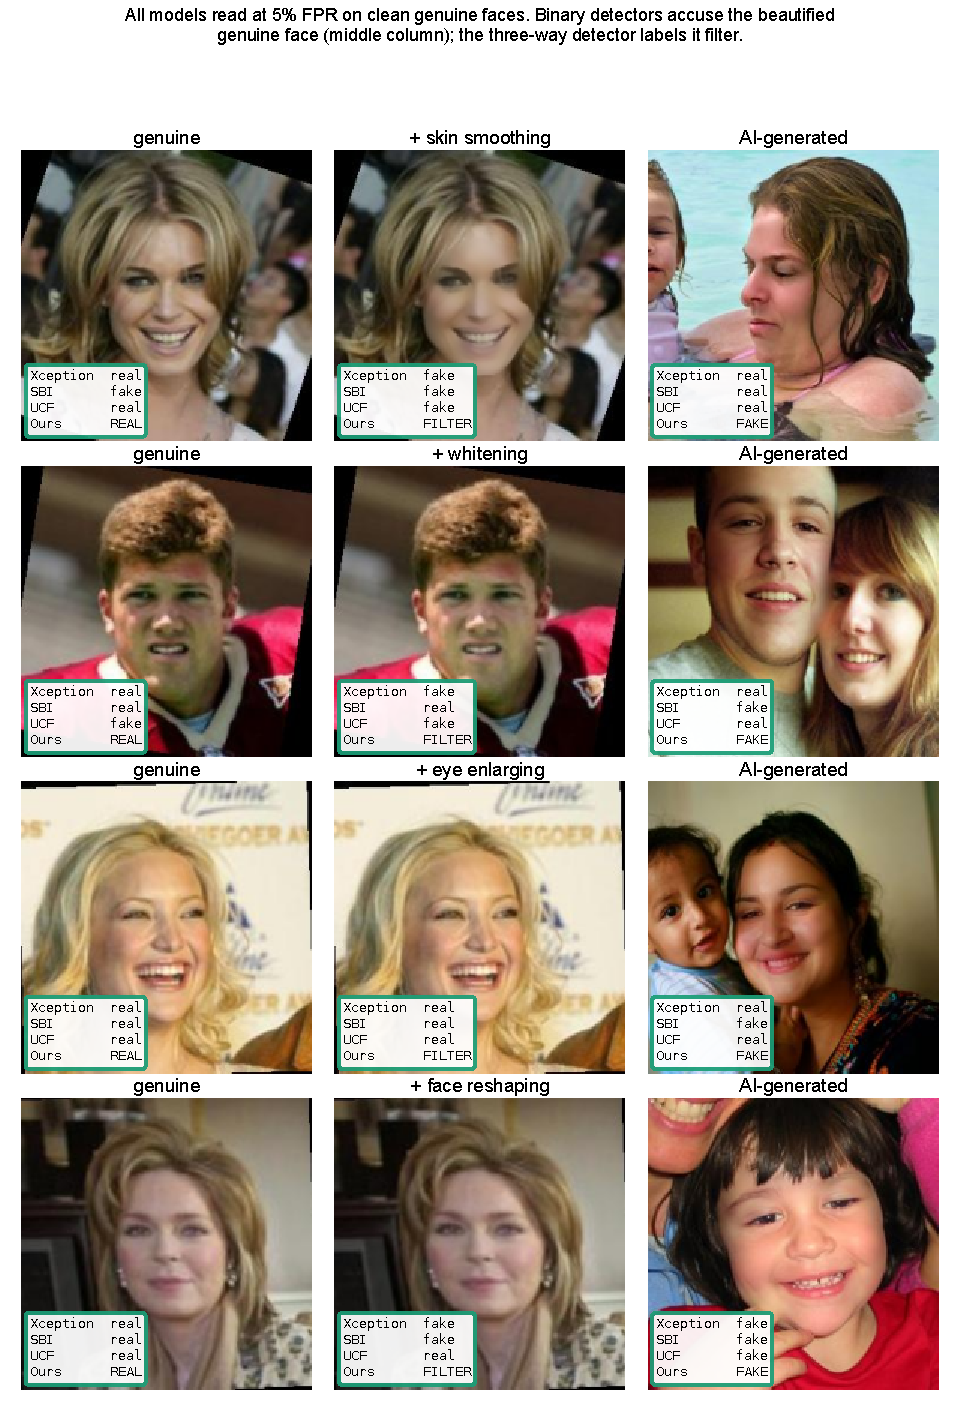
\includegraphics[width=0.78\textwidth]{fig_qualgrid.pdf}
\caption{\textbf{Qualitative comparison on identical images}, one row per filter operation.
Left: a genuine face; middle: the same face after one ordinary beauty filter; right: an
AI-generated face. Verdicts are read at each model's matched 5\,\% clean-real operating point.
The binary detectors accuse the beautified genuine faces (rows 1, 2 and 4) or miss the
generated faces (rows 1--3); the three-way detector returns \emph{filter} for the middle
column and \emph{fake} for the right. Rows are different people because the held-out set applies
exactly one operation per source photograph.}
\label{fig:qualgrid}
\end{figure*}

\begin{figure}[t]
\centering
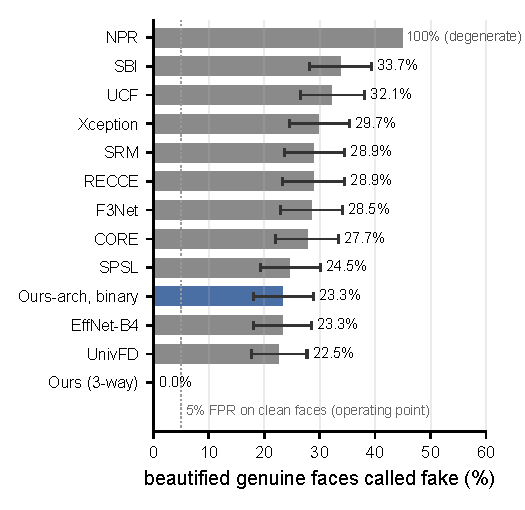
\includegraphics[width=0.9\columnwidth]{fig_fa_bar.pdf}
\caption{\textbf{False accusation of beautified genuine faces}, all models at a matched 5\,\%
FPR on the paired clean faces, with 95\,\% bootstrap intervals clustered by source image.
Our architecture under the binary recipe (blue) fails like every published detector; only the
three-way label space (green) reaches zero.}
\label{fig:fabar}
\end{figure}

\begin{figure}[t]
\centering
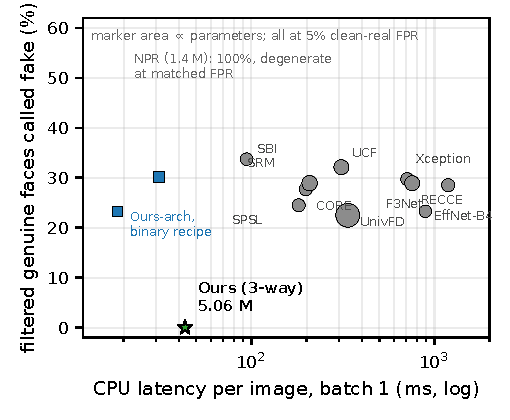
\includegraphics[width=\columnwidth]{fig_cost.pdf}
\caption{\textbf{Cost against filter-aware safety}, every model on identical images at a
matched 5\,\% clean-real FPR. Marker area is proportional to parameter count; latency is
desktop CPU, batch 1. Our three-way detector is the only model at 0\,\% false accusation and
sits at the low-latency end; our own architecture trained under the conventional binary
recipe (blue square) fails at the same rate as the published detectors.}
\label{fig:cost}
\end{figure}

Three observations follow. First, the failure is universal among binary detectors: none
falls below 22\%, a four- to sevenfold increase over its own clean false-positive rate.
Second, it is not explained by capacity, architecture family, or training corpus --- models
spanning 1.4\,M to 427.6\,M parameters, CNN and transformer backbones, and both forgery-corpus
and self-blending training regimes all fail. Third, and most directly,
\emph{our own architecture} trained under the conventional binary recipe fails at 23.3\%,
indistinguishable from the published detectors, while the identical backbone trained with a
filter class reaches 0.0\%. The difference is the label space.

A complementary observation supports the same reading: for every published detector, AUROC
computed on \emph{filtered} fakes is higher than on unfiltered fakes. They are detecting the
filter, not the forgery.

\subsection{Is the third class necessary?}
\label{sec:necessity}
Section~\ref{sec:p3} shows a binary detector \emph{does} fail; it does not yet show that it
\emph{must}. A binary detector exposes one threshold, and beauty filters displace filtered
genuine faces and filtered fakes in the same direction along it, so no threshold can serve
both. Within a binary label space there are exactly two places to put the filter class ---
with \emph{real} or with \emph{fake}. We therefore train four models that are identical in
backbone, data pool, recipe, optimiser, schedule and seed, and differ \emph{only} in the
label space: filter$\rightarrow$real, filter$\rightarrow$fake, filter absent, and three-way.

All four arms are read at a matched operating point (4.80\% false-positive rate on the 250
clean real faces) and evaluated on two paired axes: false accusation of the 249 filtered
genuine faces, and misses on the 2{,}289 filtered fakes. Figure~\ref{fig:frontier} shows the
full threshold sweep of every binary model on these two axes.

\begin{figure}[t]
\centering
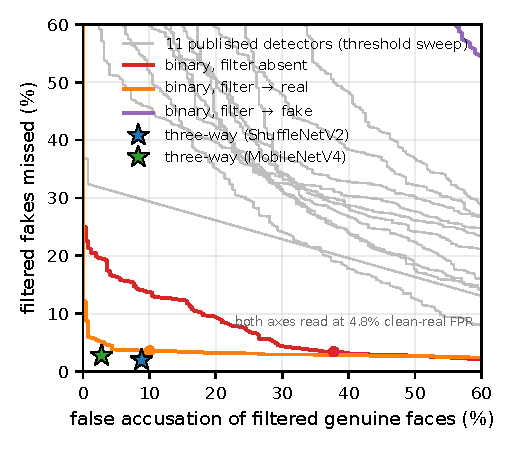
\includegraphics[width=\columnwidth]{fig_frontier.pdf}
\caption{\textbf{The binary frontier.} Each curve is one binary model's full threshold sweep
in the plane of false accusation (filtered genuine faces) against misses (filtered fakes);
grey curves are the eleven published detectors, coloured curves the three binary arms trained
on our own data, dots their matched operating points. The three-way models (stars) lie below
and to the left of every curve: no binary threshold on any model reaches both a lower
false-accusation rate and a lower miss rate.}
\label{fig:frontier}
\end{figure}

\begin{table}[t]
\caption{Four label spaces, identical in every other respect. Read at 4.80\% clean-real FPR.
Differences from the three-way model are paired bootstrap, clustered by source image.}
\label{tab:necessity}
\centering\small
\begin{tabular}{@{}lccc@{}}
\toprule
Label space & FA (filtered reals) & MISS (filtered fakes) & Clean fake rec. \\
\midrule
\textbf{Three-way} & \textbf{8.84\%} & \textbf{1.97\%} & 98.61\% \\
filter $\rightarrow$ real   & 10.04\% & 3.54\% & 98.95\% \\
filter absent               & 37.75\% & 3.41\% & 98.61\% \\
filter $\rightarrow$ fake   & 41.37\% & 76.37\% & 41.11\% \\
\bottomrule
\end{tabular}
\end{table}

The two label spaces a practitioner would actually adopt both fail. Omitting filters
entirely --- the published-detector analogue, now with our data and recipe --- gives 37.75\%
false accusation, inside the 22--33\% band of the published detectors and
$28.92$\,pp worse than the three-way model (CI $[-35.34, -22.49]$). Assigning filters to
\emph{fake} is worse still on both axes ($-32.53$ and $-74.44$\,pp, both CIs excluding zero),
because the model then treats benign retouching as forgery and loses the forgery signal
itself (clean fake recall collapses to 41\%).

The informative comparison is with the remaining option, assigning filters to \emph{real}.
That is a reasonable binary fallback and it performs reasonably: 10.04\% false accusation.
The three-way model is better on both axes, but only one difference is significant --- it
misses $1.57$\,pp fewer filtered fakes (CI $[-2.27, -0.92]$), while its $1.20$\,pp advantage
in false accusation is directional only (CI $[-5.62, +3.21]$). We state this precisely
rather than claiming a uniform win.

The pre-registered criterion is nevertheless met: sweeping the threshold of every binary arm
and of all eleven published detectors over its full range, \emph{no} threshold on \emph{any}
of them attains both a lower-or-equal false-accusation rate and a lower-or-equal miss rate
than the three-way model, and for every binary arm the gap on at least one axis excludes
zero. The verdict is therefore \textbf{necessary}: within a binary label space there is no
operating point that matches what a third class achieves.

A final observation makes the mechanism concrete. At its native decision rule the three-way
model assigns \textbf{94.78\%} of filtered genuine faces to the \emph{filter} class ---
neither accusing them nor pretending they are untouched. That third answer is what no
binary threshold can express.

\subsection{P1: composite fake-plus-filter attack}
\label{sec:p1}
On 2{,}289 filtered fakes, our end-to-end error is \textbf{2.80\%} [1.92, 3.76]. Our own
audit decomposes this: 2.11 percentage points are attributable to the filter, and the
remainder to source images the detector already fails on unfiltered; 26.6\% of source images
account for all errors. We also record a defect in the metric itself --- a single failing
source image is counted eight times, once per condition --- and report the source-level rate
alongside.

The published detectors cannot be ranked against us on this protocol, and we say so
explicitly: their AUROC on these \emph{unfiltered} fakes is 0.45--0.70 against our 0.995,
so matching recall drives their thresholds to a degenerate operating point at 89--100\% FPR.
We report this as a scope finding --- FF++- and ProGAN-trained detectors do not transfer to
this generative family zero-shot --- and not as a win.

\subsection{P2: third-party benchmark, where we lose}
\label{sec:celebdfb}
On Celeb-DF-B~\cite{libourel2024} the ordering reverses.

\begin{table}[t]
\caption{Celeb-DF-B, threshold-matched to our untreated recall.}
\label{tab:celebdfb}
\centering\small
\begin{tabular}{@{}lccc@{}}
\toprule
Model & Beautified AUROC & FA on beaut.\ reals & ASR \\
\midrule
\ours{}   & 0.524 [0.483, 0.566] & 74.1\% & 23.4\% \\
SBI       & \textbf{0.752}       & \textbf{19.3\%} & 43.7\% \\
UCF       & \textbf{0.756}       & 48.8\% & 17.6\% \\
Xception  & 0.735                & 54.8\% & \textbf{15.8\%} \\
\bottomrule
\end{tabular}
\end{table}

We are significantly worse than twelve of thirteen models on beautified AUROC. The cause is
not filter robustness: our detector calls 86--88\% of \emph{untreated} Celeb-DF real frames
fake. Grepping our own training splits explains why --- they contain 11{,}735 diffusion
fakes generated \emph{from} Celeb-DF real frames and zero Celeb-DF real frames. The cheapest
hypothesis available to the model is ``Celeb-DF-looking frame $\Rightarrow$ manipulated'',
which is precisely the observed behaviour.

We pre-registered the obvious test of that explanation and it failed. Retraining the
identical recipe with those 11{,}735 rows removed changes the untreated-real false-accusation
rate from 41.71\% to 41.45\% ($-0.26$\,pp, paired video-clustered CI $[-1.98, +1.47]$), and
neither the beautified nor the compressed real folder moves significantly either. Removing
the unpaired fakes is \emph{not} the fix.

What does move the number is the opposite intervention. Adding FaceForensics++ to training
--- which contributes 41{,}512 real \emph{video} frames --- takes the untreated-real
false-accusation rate from 87.7\% (production, whose real class is almost entirely
photographs) to 41.7\%. The operative deficiency is therefore the absence of real video
frames in the real class, not the presence of fakes derived from an unrepresented corpus.
We report the refuted hypothesis alongside the surviving one because the two are easily
confused: both are describable as ``corpus shortcut'', but only one is actionable, and the
cheap intervention suggested by the first is worthless.

No model in Table~\ref{tab:celebdfb} satisfies all three desiderata simultaneously ---
detecting the swap, not accusing beautified genuine frames, and not being evaded by the
filter. SBI is best on the second and worst on the third; Xception is the reverse.

\subsection{The standard cross-dataset protocol}
\label{sec:crossdataset}
The comparison in Table~\ref{tab:main} deliberately does not follow the field's usual
protocol, because it is asking a different question. To be comparable with the literature we
must also do what the field does: train every model on the \emph{same} corpus --- FaceForensics++
c23 --- and evaluate zero-shot on external datasets. We therefore trained our architecture on
the FF++ official training split under that protocol and evaluated it against
DeepfakeBench~\cite{yan2023bench} checkpoints on the same convention.

\begin{table}[t]
\caption{Standard protocol: all models trained on FF++ c23 only, evaluated zero-shot on
\emph{the same frames}, frame-level AUC. The published checkpoints were run by us on our
holdouts (DeepfakeBench weights; SBI authors' weights), so every row sees identical images.
Our rows are the architecture of the deployed detector trained under the literature recipe.}
\label{tab:crossdataset}
\centering\small
\begin{tabular}{@{}lrcc@{}}
\toprule
Model & Params & Celeb-DF-v2 & DFD \\
\midrule
SBI~\cite{shiohara2022}        & 17.55\,M & \textbf{0.8928} & \textbf{0.9273} \\
Xception~\cite{rossler2019}    & 20.81\,M & 0.8063 & 0.9007 \\
\midrule
Ours, MobileNetV4 dual-branch  & 3.90\,M & 0.7932--0.8325$^{\ast}$ & 0.8916--0.9062$^{\ast}$ \\
Ours, ShuffleNetV2 dual-branch & \textbf{2.55\,M} & 0.7278 & 0.8487 \\
Ours, ShuffleNetV2 spatial-only & \textbf{1.80\,M} & 0.7358 & 0.8602 \\
\midrule
\emph{Ours, production recipe} & 5.06\,M & 0.5794 & 0.6887 \\
\bottomrule
\multicolumn{4}{@{}l@{}}{\footnotesize $^{\ast}$ two seeds; the spread (3.9 points) is the
seed noise of this protocol.}
\end{tabular}
\end{table}

\begin{figure}[t]
\centering
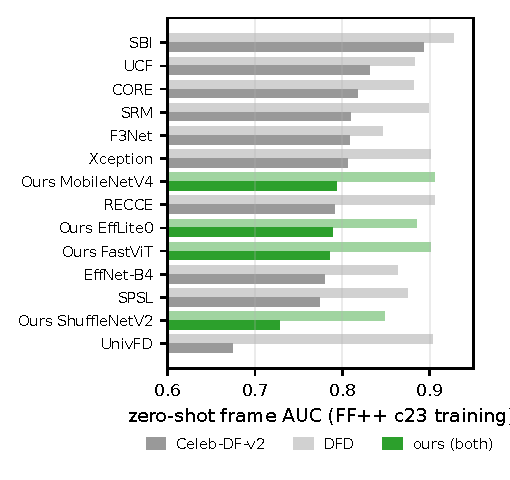
\includegraphics[width=\columnwidth]{fig_crossdataset.pdf}
\caption{\textbf{Standard cross-dataset protocol, same frames for every model.} All models
are trained on FaceForensics++ c23 only and scored zero-shot on our Celeb-DF-v2 (389 frames)
and DFD (1{,}521 frames) holdouts; published checkpoints (grey) come from DeepfakeBench and
SBI and were run by us on the identical frames. Our MobileNetV4 variant (3.90\,M) sits among
detectors of 17--47\,M parameters on both corpora; SBI remains ahead. Single seed per bar; the
seed spread measured in Sec.~\ref{sec:auxcost} is 3.9 points on Celeb-DF-v2.}
\label{fig:crossdataset}
\end{figure}

We do not win this table, and we say so. On identical frames SBI is the strongest model on
both corpora; Xception sits 7--8 points above our ShuffleNetV2 variant on Celeb-DF-v2 and 4--5
points above it on DFD, at 8--12$\times$ the parameters. Our MobileNetV4 variant (3.90\,M)
closes most of that gap --- within seed noise of Xception on both corpora --- and is the reason
Section~\ref{sec:backboneswap} tests that backbone on the safety task. The limits of even this
modest claim are: two of the four columns of the standard table; a DFD holdout of 162 of
3{,}431 videos biased toward close-up scenes because face detection fails on long shots;
Hanley--McNeil intervals without video-cluster correction; and no DFDC column, the one on which
every published method is weakest. The published numbers in the literature for Xception
(0.7365 / 0.8163) are lower than what we measure on our holdouts, which is why we report
same-frame values rather than quoting.

Two further findings belong here because they are inconvenient. First, the same architecture
trained under our production recipe scores 0.5794 and 0.6887 on these corpora --- 0.15 to 0.17
AUC \emph{below} its FF++-trained sibling. The deficit is the training corpus, not the design.
Second, the \emph{spatial-only} variant beats the dual-branch model on both external corpora
while being 29\% smaller. Combined with three earlier replications, our reading is that the
frequency branch contributes at low false-positive rates and to the filter task
(Section~\ref{sec:backbone}) but yields no net benefit for cross-dataset forgery detection.
We report this rather than presenting the branch as a uniform improvement.

\subsection{What the third class costs}
\label{sec:auxcost}
Section~\ref{sec:necessity} shows what the third class buys. Symmetry demands that we also
measure what it costs, and we pre-registered the optimistic hypothesis: that forcing the model
to separate identity-preserving from identity-replacing manipulation would penalise
non-transferable ``these pixels were edited'' cues and therefore \emph{improve} cross-dataset
forgery detection. Two arms, identical backbone (MobileNetV4), FF++ training frames, recipe
and seed, differing only in whether 12{,}000 retouched images are added as a third class:

\begin{table}[t]
\caption{Cost of the third class. Paired image bootstrap, the same resampled indices scored
for both arms, $N_B = 10{,}000$.}
\label{tab:auxcost}
\centering\small
\begin{tabular}{@{}lccc@{}}
\toprule
Zero-shot holdout & Binary & + filter class & $\Delta$ (95\,\% CI) \\
\midrule
Celeb-DF-v2 & \textbf{0.8325} & 0.7955 & $-0.0370$ $[-0.0687, -0.0061]$ \\
DFD & \textbf{0.8916} & 0.8739 & $-0.0177$ $[-0.0314, -0.0044]$ \\
\bottomrule
\end{tabular}
\end{table}

The hypothesis is refuted, significantly and on both corpora. In-domain validation is
unchanged (F1 0.9207 versus 0.9206), so the cost falls specifically on transfer. We therefore
state the design's trade-off with numbers rather than rhetoric: the third class removes the
false-accusation failure mode entirely, and no binary label space matches it on both safety
axes, at a cost of \textbf{1.8--3.7 AUC points} of zero-shot cross-dataset forgery detection.

One further measurement constrains every single-seed comparison in this paper, including our
own. The binary arm here is the same configuration as the MobileNetV4 row of
Table~\ref{tab:crossdataset}, differing only in seed, and it scores 0.8325 against that row's
0.7932 on Celeb-DF-v2 --- a 3.93-point spread between two seeds of one configuration on a
389-frame holdout, larger than most gaps we report between \emph{methods}. Cross-dataset
rankings on this holdout should be read as approximate, and we do not claim ordinal
superiority over any baseline on Celeb-DF-v2 on the strength of a single seed.

\subsection{Does a better detection backbone cost safety?}
\label{sec:backboneswap}
Section~\ref{sec:auxcost} shows the third class trades generalisation for safety. The
complementary worry is whether the reverse holds --- whether the backbones that detect
forgeries better would give the safety back. Every backbone comparison we ran
(Table~\ref{tab:backbone} and Section~\ref{sec:crossdataset}) measured only detection, so the
substitution was untested. We therefore retrained the three-way model with MobileNetV4 in
place of ShuffleNetV2, holding data, label space, recipe, schedule and seed fixed.

\begin{table}[t]
\caption{Backbone substitution on the filter-aware task, read at the same matched operating
point. Paired bootstrap clustered by source image, $N_B = 10{,}000$.}
\label{tab:backboneswap}
\centering\small
\begin{tabular}{@{}lccc@{}}
\toprule
& ShuffleNetV2 & MobileNetV4 & $\Delta$ (95\,\% CI) \\
\midrule
FA (filtered reals)   & 8.84\,\% & \textbf{2.81\,\%} & $-6.43$ $[-10.44, -2.41]$ \\
MISS (filtered fakes) & \textbf{1.97\,\%} & 2.71\,\% & $+0.74$ $[-0.22, +1.71]$ \\
Clean fake recall     & 98.61\,\% & \textbf{100.00\,\%} & --- \\
\bottomrule
\end{tabular}
\end{table}

On the matched frontier the better detection backbone does \emph{not} trade away safety: it
cuts false accusation by 6.43 points with the interval excluding zero, leaves the miss rate
statistically unchanged, and reaches perfect clean-fake recall, while also being faster on CPU.
At the native three-way rule it routes 95.58\,\% of beautified genuine faces to \emph{filter}
and keeps 99.63\,\% fake recall. A second training seed replicates the frontier result
(FA 2.81\,\%, MISS 2.49\,\%, $\Delta$FA $-6.02$ $[-10.04, -2.01]$, $\Delta$MISS $+0.52$
$[-0.48, +1.57]$).

The full release battery, however, is not a clean win. Read at its own native rule, the
flat MobileNetV4 model calls 11.36\,\% of composite fake-plus-filter images \emph{filter}
instead of \emph{fake} (protocol P1), against 7.25\,\% for the flat ShuffleNetV2 twin and
2.80\,\% for the deployed hierarchical detector; and its recall on the third-party Alibaba
retouching set drops to 72.4\,\% (ShuffleNetV2 twin 99.7\,\%). The other gates hold
(AIGuard-unseen AUROC 0.827 vs.\ 0.841 for the deployed model; CelebA 100\,\%; StyleGAN2
99.9\,\%; Shadow real recall 94.3\,\% vs.\ 74.9\,\%, all read by the same harness). Because the flat label space by itself raises the P1 error from 2.80
to 7.25\,\%, we also retrained MobileNetV4 inside the production hierarchy on the production
splits (ImageNet initialisation, single seed). It fails six of eight release gates --- P1 error
15.1\,\%, Alibaba recall 57.3\,\%, held-out AUROC 0.765, True Test fake 98.5\,\% and filter
89.6\,\% --- and is worse than its flat sibling on the two safety gates, so the failure is the
backbone under our data, not the label space. We read the two results together: the frontier
gain is real at a matched operating point on the filters we generate, and does not transfer
to composite attacks or a third-party retouching algorithm at the native rule. The deployed
system therefore stays on ShuffleNetV2; the property this paper is about comes from the label
space, not from the backbone.

\subsection{Why the two protocols are both needed}
Table~\ref{tab:crossdataset} and Table~\ref{tab:main} answer different questions, and neither
subsumes the other. The standard protocol controls the training corpus and asks which model
generalises better at forgery detection; on it we claim parity at far lower cost. The
filter-aware protocol asks whether a label space that omits retouching can be safe at all;
there, controlling the corpus is achieved differently --- by training \emph{our own architecture}
under the conventional binary recipe (row 2 of Table~\ref{tab:main}), which fails at 23.3\%
exactly like the published detectors, and by the four-arm experiment of
Section~\ref{sec:necessity} in which only the label space varies. A reader who objects that we
win Table~\ref{tab:main} because we trained on filters is making the point we are making: no
binary detector can be trained out of this failure, because its label space has nowhere to put
the answer.

\subsection{Cross-dataset frontier of the deployed model}
\label{sec:frontier}
Our detector's zero-shot frame AUROC on the FaceForensics++ official test split is 0.575.
The same architecture trained on the FF++ official training split reaches \textbf{0.9155},
which locates the deficit in training-data coverage rather than in the architecture.
Adding FF++ data to production training raises FF++ AUROC to 0.81--0.83 across four
independent runs, but degrades the P1 safety metric from 2.80\% to 5.9--6.7\%. We
characterise this as a genuine trade-off frontier for this backbone, measured at eight
operating points, rather than as a solved problem: three standard continual-learning
remedies (learning-without-forgetting, a family-factorised head, and parameter anchoring)
each failed to clear both bars, and the one candidate that appeared to succeed on a single
seed was refuted by its own pre-registered second seed.

\subsection{Explainability}
\label{sec:xai}
We report a null result. Under RISE deletion and insertion tests against a fixed
centre-Gaussian control, our production Grad-CAM++ maps are statistically indistinguishable
from the prior that ``the face is in the middle'' (Layer 1 deletion AUC 0.787 versus 0.787,
$\Delta = 0.000$ [$-0.004$, $+0.004$]), and they fail the Adebayo classifier-head
randomisation check (Spearman 0.83--0.97 after re-initialisation). We therefore make no
faithfulness claim for saliency. The trained patch evidence head passes four of six
pre-registered faithfulness cells; the two it fails are also failed by a ground-truth-mask
oracle, which indicates the cells are unattainable rather than the head deficient.

\subsection{Vision-language model as a control}
\label{sec:vlm}
Following the project's original plan, we fine-tune Qwen2-VL-7B with LoRA
(10.1\,M trainable parameters) on 32{,}961 images --- 23{,}961 FakeClue face images with
natural-language artifact annotations plus 9{,}000 of our own three-class images --- and
evaluate it on the same 769-image held-out set. It reaches 20.8\% recall on real faces
(192 of 250 genuine faces are called \emph{filter}), 80.0\% on fakes and 77.5\% on filtered
faces, for roughly 59.9\% overall. A 7\,B multimodal model fine-tuned on this task therefore
does not approach a 5.06\,M-parameter specialised detector, which supports treating it as a
teacher or control rather than as the deployed model.
On FakeClue's own held-out face split the same teacher classifies 99.67\% correctly
[99.0, 100.0] and its generated artifact descriptions reach ROUGE-L 0.462 against the
dataset's reference clues. The 40-point gap between 99.67\% in-domain and 59.9\% on our
held-out set is the corpus-shortcut pattern again, now in a 7\,B multimodal model: it has
learned the corpus, and the fluency of its explanations is no evidence that it has learned
the task.

Distilling the teacher's artifact vocabulary into the deployed model is nonetheless cheap.
A single linear layer of \textbf{35{,}854 parameters} on the frozen concatenated features of
the production Layer 1 and Layer 2 --- no backbone change, no fine-tuning of any production
weight --- recovers eight of the fourteen artifact concepts at F1 0.729--0.869 on held-out
FakeClue faces (over-smoothed skin, eye reflections, pupil mismatch, lip bleeding, jaw
contour, inconsistent lighting, pixelated nostrils, hair blur).

We failed our own pre-registered bar and report why. The bar was macro-F1 $\ge 0.70$ over all
fourteen tags and the result is 0.4758. The four \emph{filter} tags have zero support on the
evaluation set, because FakeClue contains no retouching class at all; they score zero by
construction and remove 28.6 points from a fourteen-tag mean. Over the ten tags with any
support the figure is 0.6662, and over the eight with more than a hundred examples it is
0.8188. The bar was specified against a test set that structurally cannot measure four of its
own targets --- our specification error, not a property of the distilled head --- and the
correct evaluation, on a set containing filtered faces with known operations, remains to be
run, as does the deletion-based faithfulness check that was declared alongside it.

\subsection{Deployment}
\label{sec:deploy}
The frequency branch initially made the model \emph{undeployable}: \texttt{torch.fft} exports
to an operator that mobile runtimes cannot parse, so the model failed to load at all. We
rewrote the fixed-size DFT as a constant matrix product with the shift folded into the
constants. This is mathematically equivalent, requires no retraining, and reuses the existing
weights; the exported graph contains only standard operators.

The exported fp32 model occupies \SI{20.91}{\mega\byte} for the two classification stages
(\SI{25.75}{\mega\byte} including the artifact classifier) and reproduces the PyTorch
decision on 769 of 769 held-out images. Integer quantisation is not usable for the frequency
branch and we explain why rather than omitting it: the log-magnitude spectrum spans a
dynamic range of $7.6\times10^{9}$, so per-tensor quantisation collapses 98\% of spectral
bins to zero and the network emits NaN.

\TODO{on-device measurement. Two paths are prepared and neither is yet executed:
(i) a native Android build mirroring the production decision path, and (ii) a browser
build running the same ONNX graphs through WebAssembly, servable to a phone over the local
network. Report the measured device, latency percentiles and model sizes here, or state
plainly that no on-device measurement was made. The previous draft reported device
measurements that could not be traced to any artifact and they have been removed.}

% ============================================================================
\section{Limitations}
\label{sec:limits}
% ============================================================================

\begin{itemize}
\item \textbf{Filter generalisation.} Our advantage in Table~\ref{tab:main} is demonstrated
      on our own four filter algorithms, each with a single fixed parameter setting. On
      third-party beautification presets we lose (Section~\ref{sec:celebdfb}). The
      false-accusation result should be read as evidence that the third class removes a
      structural failure mode, not that our particular detector generalises across filters.
\item \textbf{Filter sub-type classification across algorithms.} The artifact head reaches
      high accuracy in-domain but is weak across unseen retouching implementations; we
      attribute this to every training filter having a single parameterisation, and three
      attempted remedies did not fix it.
\item \textbf{Explainability.} No faithfulness claim is made for saliency maps
      (Section~\ref{sec:xai}), and no human evaluation of explanation quality was conducted.
\item \textbf{Cross-dataset detection.} We do not compete with cross-domain state of the art;
      Section~\ref{sec:frontier} reports the frontier honestly.
\item \textbf{Backbone choice.} ShuffleNetV2 was selected on the criterion in
      Table~\ref{tab:backbone}, and that criterion was too narrow. MobileNetV4 is better on
      every axis we have since measured --- FF++ in-domain (0.9383 vs 0.9155), both
      cross-dataset holdouts, CPU latency (14.1 vs 19.0\,ms despite more parameters), and
      the filter-safety axes of Section~\ref{sec:backboneswap} --- and it is the backbone this
      project's own proposal specified before we deviated. The deployed system reported here
      still uses ShuffleNetV2; switching requires a second seed and the full gate battery on
      the hierarchical architecture, which is left as the immediate next step rather than
      claimed.
\item \textbf{On-device evidence.} See Section~\ref{sec:deploy}.
\end{itemize}

% ============================================================================
\section{Conclusion}
% ============================================================================

Beauty filters are neither authentic capture nor forgery, and forcing them into a binary
taxonomy produces a specific, measurable harm: at a matched operating point, filtering a
genuine face raises the false-accusation rate of every published detector we tested to
between 22.5\% and 33.7\%. Treating filtering as its own class removes that failure mode
entirely on the same images, and does so at 5.06\,M parameters and \SI{43}{\milli\second}
per image. The same benchmark shows where the approach does not yet reach --- a third-party
beautification benchmark on which we are outperformed, traced to a countable shortcut in
our own training corpus. We release the per-image scores for all thirteen models so that
the filter-aware setting can be evaluated by others under the same protocol.

% ============================================================================
\begin{thebibliography}{00}
\bibitem{groh2022} M. Groh \emph{et al.}, ``Deepfake detection by human crowds, machines,
and machine-informed crowds,'' \emph{PNAS}, 2022.
\bibitem{saeed2025} S. Saeed \emph{et al.}, ``On the effect of beautification filters on
deepfake detectors,'' arXiv:2509.07178, 2025.
\bibitem{rossler2019} A. R\"ossler \emph{et al.}, ``FaceForensics++: Learning to detect
manipulated facial images,'' in \emph{ICCV}, 2019.
\bibitem{qian2020} Y. Qian \emph{et al.}, ``Thinking in frequency: Face forgery detection by
mining frequency-aware clues,'' in \emph{ECCV}, 2020.
\bibitem{liu2021} H. Liu \emph{et al.}, ``Spatial-phase shallow learning: Rethinking face
forgery detection in frequency domain,'' in \emph{CVPR}, 2021.
\bibitem{luo2021} Y. Luo \emph{et al.}, ``Generalizing face forgery detection with
high-frequency features,'' in \emph{CVPR}, 2021.
\bibitem{cao2022} J. Cao \emph{et al.}, ``End-to-end reconstruction-classification learning
for face forgery detection,'' in \emph{CVPR}, 2022.
\bibitem{yan2023ucf} Z. Yan \emph{et al.}, ``UCF: Uncovering common features for
generalizable deepfake detection,'' in \emph{ICCV}, 2023.
\bibitem{ni2022} Y. Ni \emph{et al.}, ``CORE: Consistent representation learning for face
forgery detection,'' in \emph{CVPRW}, 2022.
\bibitem{shiohara2022} K. Shiohara and T. Yamasaki, ``Detecting deepfakes with self-blended
images,'' in \emph{CVPR}, 2022.
\bibitem{ojha2023} U. Ojha \emph{et al.}, ``Towards universal fake image detectors that
generalize across generative models,'' in \emph{CVPR}, 2023.
\bibitem{tan2024} C. Tan \emph{et al.}, ``Rethinking the up-sampling operations in CNN-based
generative network for generalizable deepfake detection,'' in \emph{CVPR}, 2024.
\bibitem{yan2023bench} Z. Yan \emph{et al.}, ``DeepfakeBench: A comprehensive benchmark of
deepfake detection,'' in \emph{NeurIPS D\&B}, 2023.
\bibitem{ying2023} Q. Ying \emph{et al.}, ``RetouchingFFHQ: A large-scale dataset for
fine-grained face retouching detection,'' in \emph{ACM MM}, 2023.
\bibitem{libourel2024} A. Libourel \emph{et al.}, ``A case study on how beautification
filters can fool deepfake detectors,'' in \emph{IWBF}, 2024.
\bibitem{xu2025} Z. Xu \emph{et al.}, ``FakeShield: Explainable image forgery detection and
localization via multi-modal large language models,'' in \emph{ICLR}, 2025.
\bibitem{wen2025} S. Wen \emph{et al.}, ``Spot the fake: Large multimodal model-based
synthetic image detection with artifact explanation,'' arXiv:2503.14905, 2025.
\bibitem{chattopadhyay2018} A. Chattopadhyay \emph{et al.}, ``Grad-CAM++: Generalized
gradient-based visual explanations for deep convolutional networks,'' in \emph{WACV}, 2018.
\bibitem{adebayo2018} J. Adebayo \emph{et al.}, ``Sanity checks for saliency maps,'' in
\emph{NeurIPS}, 2018.
\bibitem{dang2020} H. Dang \emph{et al.}, ``On the detection of digital face manipulation,''
in \emph{CVPR}, 2020.
\bibitem{ma2018} N. Ma \emph{et al.}, ``ShuffleNet V2: Practical guidelines for efficient
CNN architecture design,'' in \emph{ECCV}, 2018.
\end{thebibliography}

\end{document}
